\section{Siti di misura e lunghezze d'onda impiegate}
\todo{sistemare riferimenti bibliografia (preferibilmente no treccani)}
\subsection{Assorbimento dell'energia luminosa e lunghezze d'onda}
Il fenomeno dell'assorbimento rappresenta una riduzione dell'energia luminosa. Nei tessuti umani questo è dovuto principalmente a due sostanze \cite{Lister2012}: 
\begin{itemize}
\item L'emoglobina, spesso indicata con la sigla Hb, è una proteina contenente ferro in grado di combinarsi in modo reversibile con l’ossigeno molecolare \cite{SilverthornDeeUnglaub2020Fu:u}. Essa presenta, all'interno nella regione della luce visibile, tre picchi di assorbimento. Il primo (noto anche come Picco di Soret), che è quello dominante, si riferisce alla regione blu dello spettro, gli altri due invece si possono distinguere nella regione giallo-verde, avente lunghezza d'onda tra i 500 e 600 nm. Questi tre picchi combinati danno all'emoglobina un colore rosso.
\item La melanina è contenuta sotto forma di granuli nelle cellule dello strato basale dell’epidermide \cite{SilverthornDeeUnglaub2020Fu:u}. Questa assorbe principalmente le lunghezze d'onda più corte, quindi uno spettro di assorbimento che decresce gradualmente dall'ultravioletto fino all'infrarosso. In realtà la melanina presenta una complessità elevata; infatti, la sua struttura non è ancora bene nota, ed è in corso di studio e oggetto di dibattito scientifico.
\end{itemize}
Un altro elemento di cui tener conto è l'acqua che in realtà presenta una basso assorbimento nella regione visibile, mentre assorbe la luce nel regime ultravioletto e del lontano infrarosso. Le regioni di luce che riescono ad attraversare maggiormente i tessuti umani sono quindi quella rossa e del vicino infrarosso, che le rende fonti utilizzabili per applicazioni di fotopletismografia.
\begin{figure}[h]
	\centering
	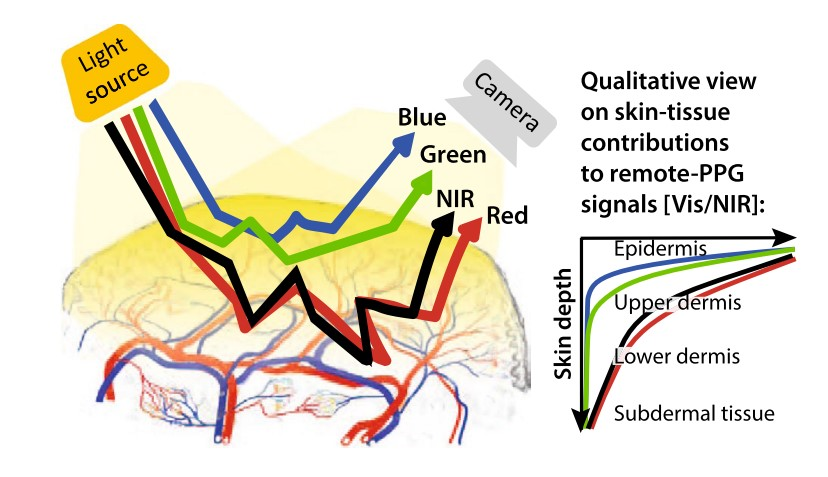
\includegraphics[width=0.7\linewidth]{ImageFiles/Fotopletismografia/PenetrazioneLuce}
	\caption{Profondità nel tessuto raggiunta dalla luce in funzione della lunghezza d'onda.}
	\label{fig:PenetrazioneLuce}
\end{figure}
La profondità nel tessuto umano che si può raggiungere dipende dalla lunghezza d'onda ma anche dalla distanza tra la sorgente luminosa e il foto-rilevatore. Le sorgenti rossa e infrarossa permettono acquisizioni a maggiore profondità nel tessuto. La luce verde invece, per via dell'emoglobina e della deossiemoglobina, viene assorbita in quantità superiore a quella infrarossa \cite{Lee2021}. Infatti, nelle zone in cui il sangue pulsa attraverso la pelle si rileva una variazione tra luce emessa e riflessa maggiore per la regione verde rispetto a quella infrarossa. Questa caratteristica per mettere di avere un rapporto segnale-rumore (Signal to Noise Ratio), per rilevazioni con luce verde, superiore a quello ottenibile con luce infrarossa. Pertanto, la luce verde risulta più adatta per misure superficiali come la variazione del flusso sanguigno superficiale \cite{Youssef2020}.
\subsection{Siti di misura}
La scelta del sito di misura risulta ancora oggi oggetto di discussione dal momento che è difficile esibire una zona del corpo "migliore" per acquisizioni fotopletismografiche. In realtà, la scelta va fatta in base alla tipologia di applicazione e alla qualità di acquisizione che si reputa accettabile.
\begin{figure}[h]
	\centering
	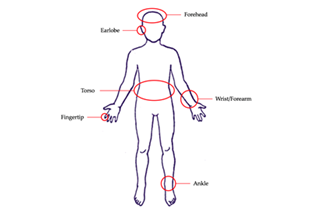
\includegraphics[width=0.7\linewidth]{ImageFiles/Fotopletismografia/ZoneAcquisizione}
	\caption{I principali siti di misura impiegati per segnali PPG.}
	\label{fig:ZoneAcquisizione}
\end{figure}
Tuttavia ci sono alcune zone che vengono privilegiati per il posizionamento dei sensori PPG:
	\paragraph{Polpastrello}
	 I polpastrelli sono la zona più comune per acquisizioni fotopletismografiche ed rappresentano un'area del corpo ricca di capillari e con una bassa concentrazione di melanina, quindi particolarmente adatta a misure in profondità con luce rossa e infrarossa. Il segnale acquisito riflette i movimenti del sangue che va dal cuore alle punte delle dita \cite{Elgendi2012}.
	 \paragraph{Polso}
	 Un primo tipo di acquisizioni sul polso è quello sulla parte superiore (postero-esterno), dove si ha maggiore presenza di capillari sanguigni. Per questo tipo di misura si impiega principalmente la luce verde.
	 Il secondo tipo di acquisizione invece è quello che coinvolge la parte inferiore(antero-interna), dove si ha il passaggio delle arterie ulnare e radiale. Risultano quindi adatte le luci rossa e infrarossa. Questa tipologia di acquisizione permette l'ottenimento di risultati migliori e più accurati.
	 Tuttavia, nei dispositivi commerciali, prevale l'acquisizione sulla faccia postero-esterna poiché sono più agevoli da indossare.
	 Un limite di queste misure è la presenza di disturbi legati al movimento del braccio che però possono essere ridotti tramite l'integrazione di una piattaforma inerziale nel sensore PPG \cite{Ghamari2018}.
	 \paragraph{Fronte}
 	 La fronte è un sito utilizzato tipicamente per la misura della saturazione arteriosa di ossigeno, si tratta anche di una regione ricca di arterie che si diramano dalla carotide interna \cite{Abay2019}, le misure in questa zona offrono quindi una buona qualità e affidabilità del segnale. Le acquisizioni sulla fronte sono anche meno sensibili ai disturbi legati al movimento ed è una posizione più accessibile rispetto ai polpastrelli.
 	 \paragraph{Orecchio}
	 I lobi delle orecchie sono un altro sito molto comune per acquisizioni fotopletismografiche. Questa zona ha un basso contenuto di cartilagine e una elevata affluenza di sangue, queste caratteristiche permettono di ottenere dei segnali di buona qualità. Anche per il lobi delle orecchie si ha meno vulnerabilità agli artefatti dovuti al movimento e offrono una posizione comoda, infatti, i dispositivi di questo tipo sono altamente indossabili \cite{Ghamari2018}\cite{Vescio2018}.

 